\subsection{Experimentación y gráficos.}

\vspace*{0.3cm}

En esta sección trataremos de encontrar, entre las heurísticas anteriormente estudiadas, aquella que tenga el mejor balance entre calidad de solución y performance. 

En el caso de la búsqueda local, se consideró tomar la solución inicial provista por la heurística golosa, y mejorarla mediante la Vecindad 2. En el caso de GRASP, se tomó como criterio de parada la ejecución de 10 iteraciones sin mejoras, y generar la RCL con los nodos candidatos cuya cantidad de vecinos ``libres'' sea no menor a un $10 \%$ de la cantidad de vecinos ``libres'' del mejor candidato.

Plantearemos entonces, experimentos que nos permitan observar cómo se desenvuelven nuestros algoritmos, evaluando instancias de tipo $circuito$, $estrella$, $galaxia$ y $aleatorio$.
 
\subsubsection{Circuitos}

Se generaron 40 $circuitos$ con entre 10 y 50 nodos.  El orden de los nodos fue aleatorizado para no depender de un rotulado en particular.

\paragraph{Performance} 

El gráfico obtenido con las mediciones de tiempo es el que se muestra en la Figura \ref{fig:5A}.

\begin{figure}[htb]
	\begin{center}
    		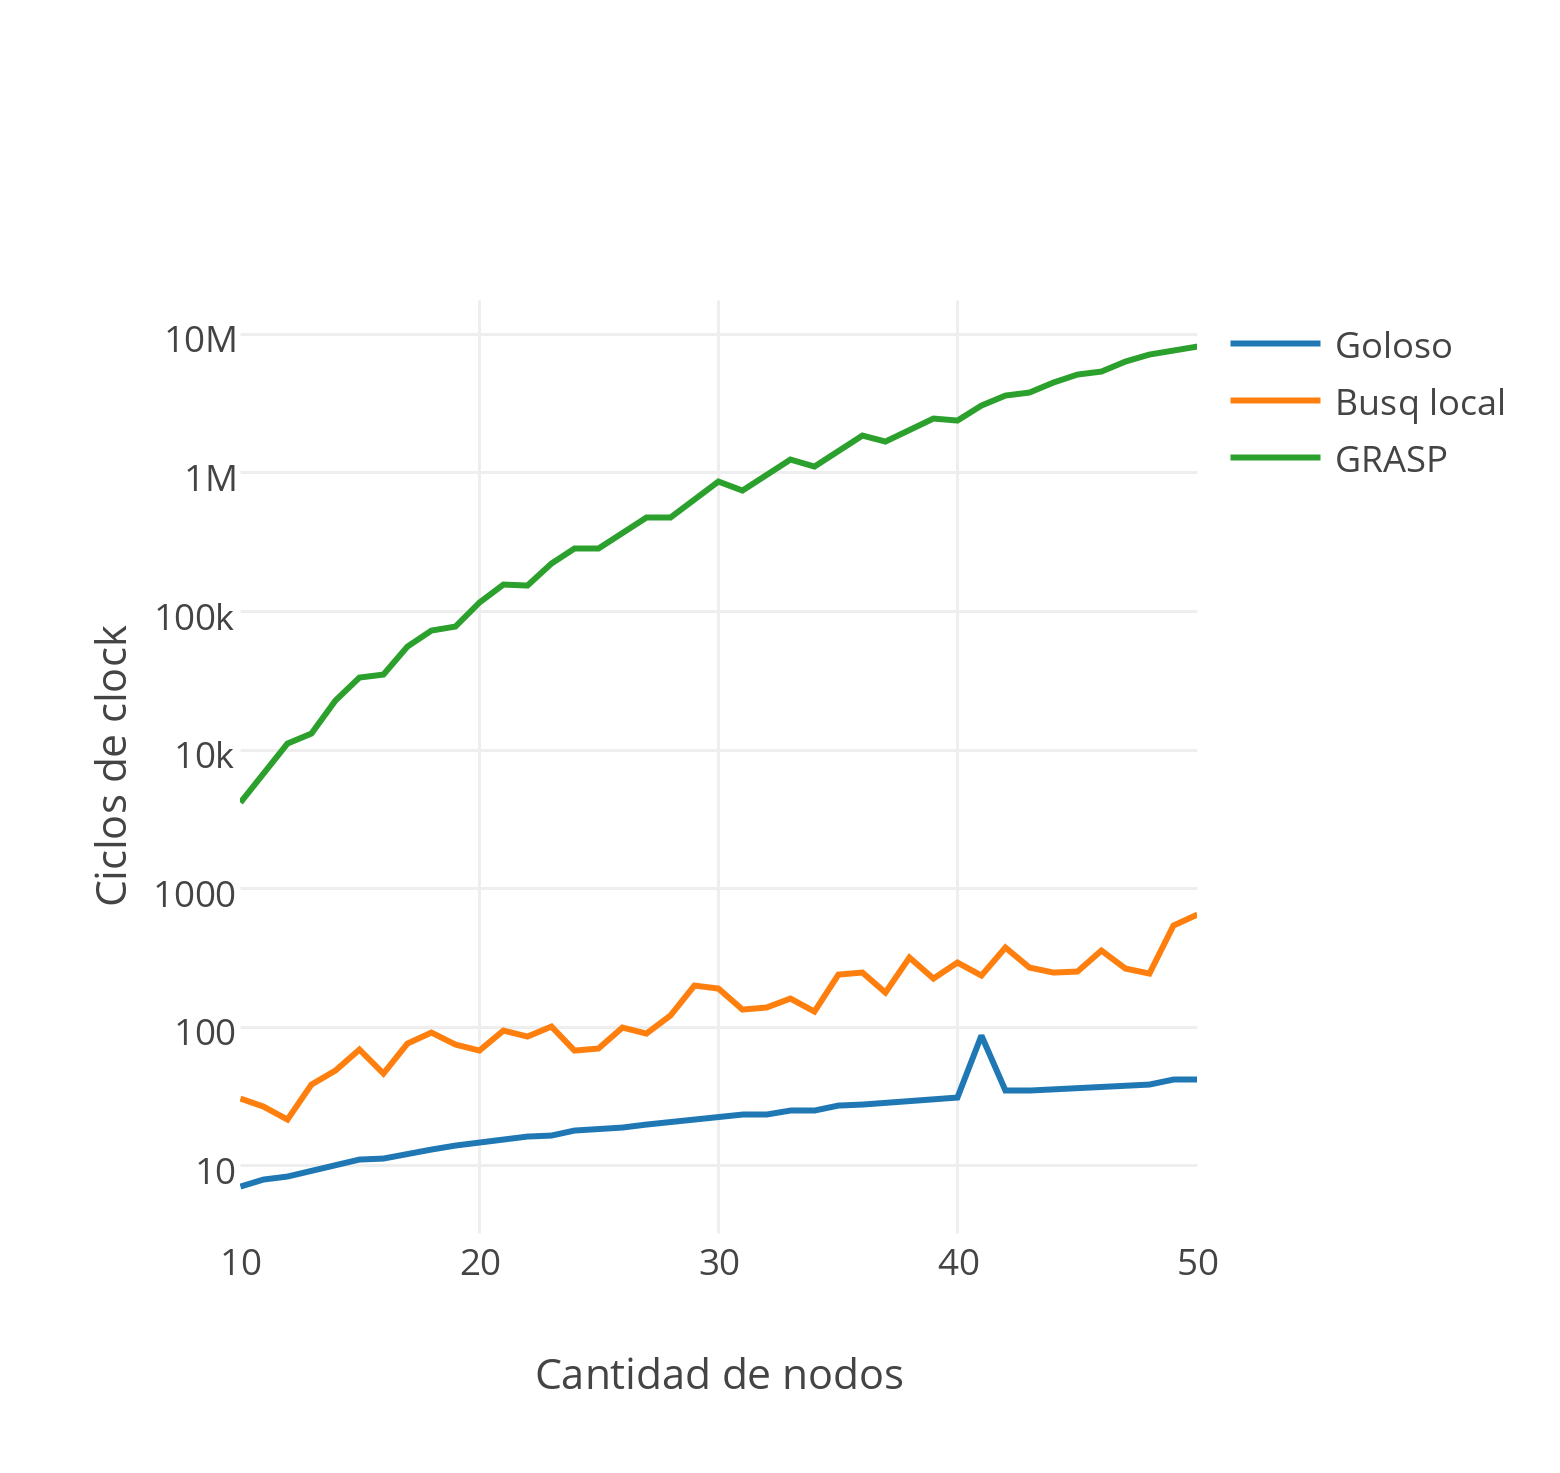
\includegraphics[scale=0.8]{imagenes/final-circuitos.png}
	\end{center}
	\caption{Comparación - Circuitos}\label{fig:5A}
\end{figure}
%\FloatBarrier

La Figura muestra claramente que el tiempo de ejecución del algoritmo goloso es menor a los otros dos algoritmos, el tiempo de ejecución de la búsqueda local es algo mayor al goloso, y que el tiempo de ejecución de GRASP es mucho mayor a los otros dos.

\paragraph{Calidad} Se ha comparado el tamaño de las soluciones halladas con el tamaño de la solución exacta.  Los porcentajes de desaciertos sobre el total de instancias evaluadas son los siguientes:

\begin{verbatim}
Goloso: 85.37%
Búsqueda Local: 53.65%
GRASP: 4.87%
\end{verbatim}

El algoritmo goloso muestra una tasa de error muy grande, la búsqueda local tiene un porcentaje de error menor pero bastante significativo, y GRASP muestra una tasa de error mínima.

\subsubsection{Estrellas}

Se generaron 60 grafos $estrellas$ con entre 20 y 60 nodos.

\paragraph{Performance}

La Figura \ref{fig:5B} muestra los resultados obtenidos respecto al tiempo de ejecución. La Figura muestra claramente que el tiempo de ejecución del algoritmo goloso es menor a los otros dos algoritmos, el tiempo de ejecución de la búsqueda local es algo mayor al goloso, y que el tiempo de ejecución de GRASP es mucho mayor a los otros dos.

\begin{figure}[htb]
	\begin{center}
    		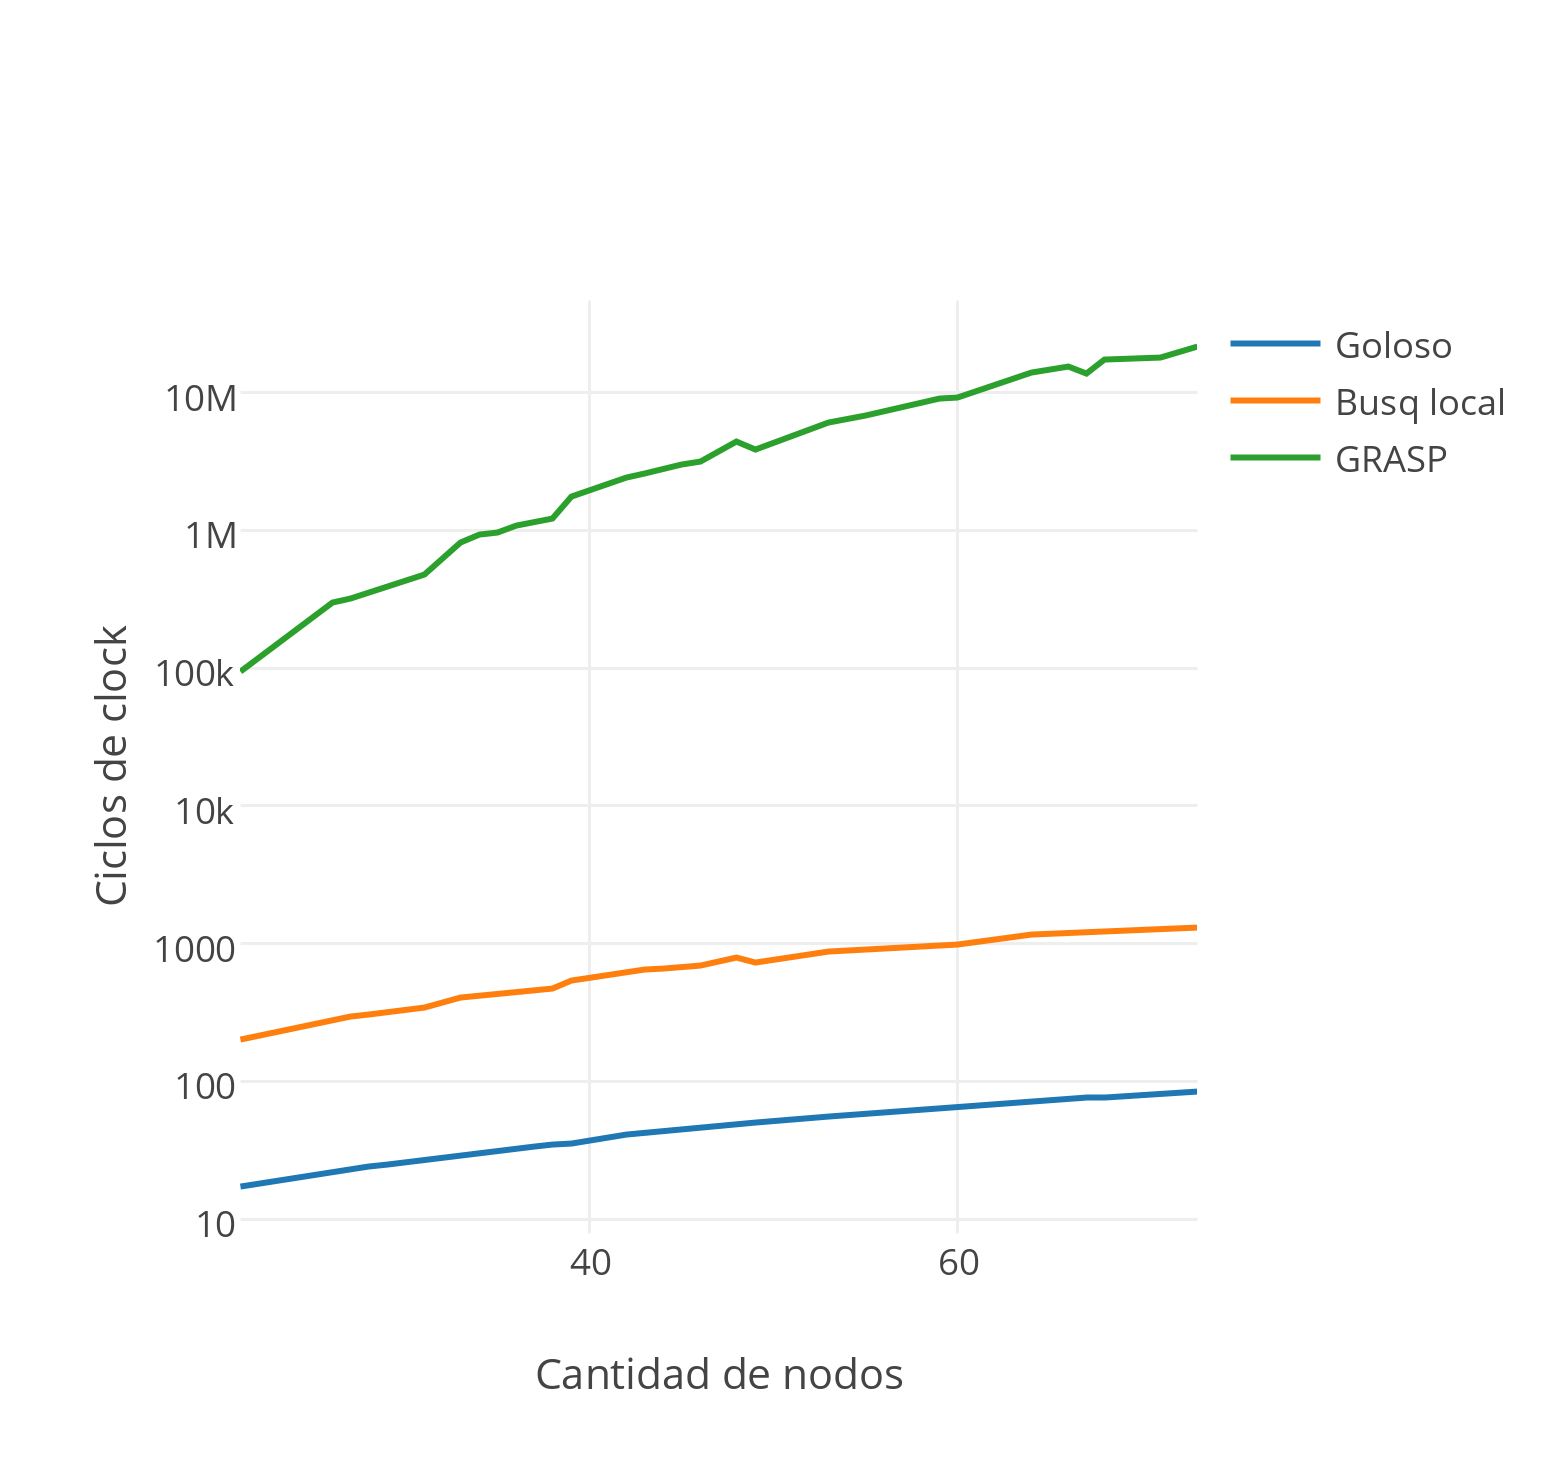
\includegraphics[scale=0.8]{imagenes/final-estrellas.png}
	\end{center}
	\caption{Comparación - Estrellas}\label{fig:5B}
\end{figure}
%\FloatBarrier

\paragraph{Calidad} Se ha comparado el tamaño de la solución obtenida con el tamaño de la solución exacta. Los porcentajes de desaciertos sobre el total de instancias evaluadas son los siguientes:

\begin{verbatim}
Goloso: 100%
Búsqueda Local: 0%
GRASP: 4%
\end{verbatim}

Podemos observar que el algoritmo goloso nunca encuentra una solución exacta, mientras que la búsqueda local siempre la encuentra y GRASP tiene un porcentaje de desaciertos mínimo.

\subsubsection{Galaxias}

Se generaron 30 grafos $galaxia$ con entre 35 y 90 nodos.

\paragraph{Performance}

La Figura \ref{fig:5C} muestra los resultados obtenidos respecto al tiempo de ejecución. La Figura muestra claramente que el tiempo de ejecución del algoritmo goloso es menor a los otros dos algoritmos, el tiempo de ejecución de la búsqueda local es algo mayor al goloso, y que el tiempo de ejecución de GRASP es mucho mayor a los otros dos.

\begin{figure}[htb]
	\begin{center}
    		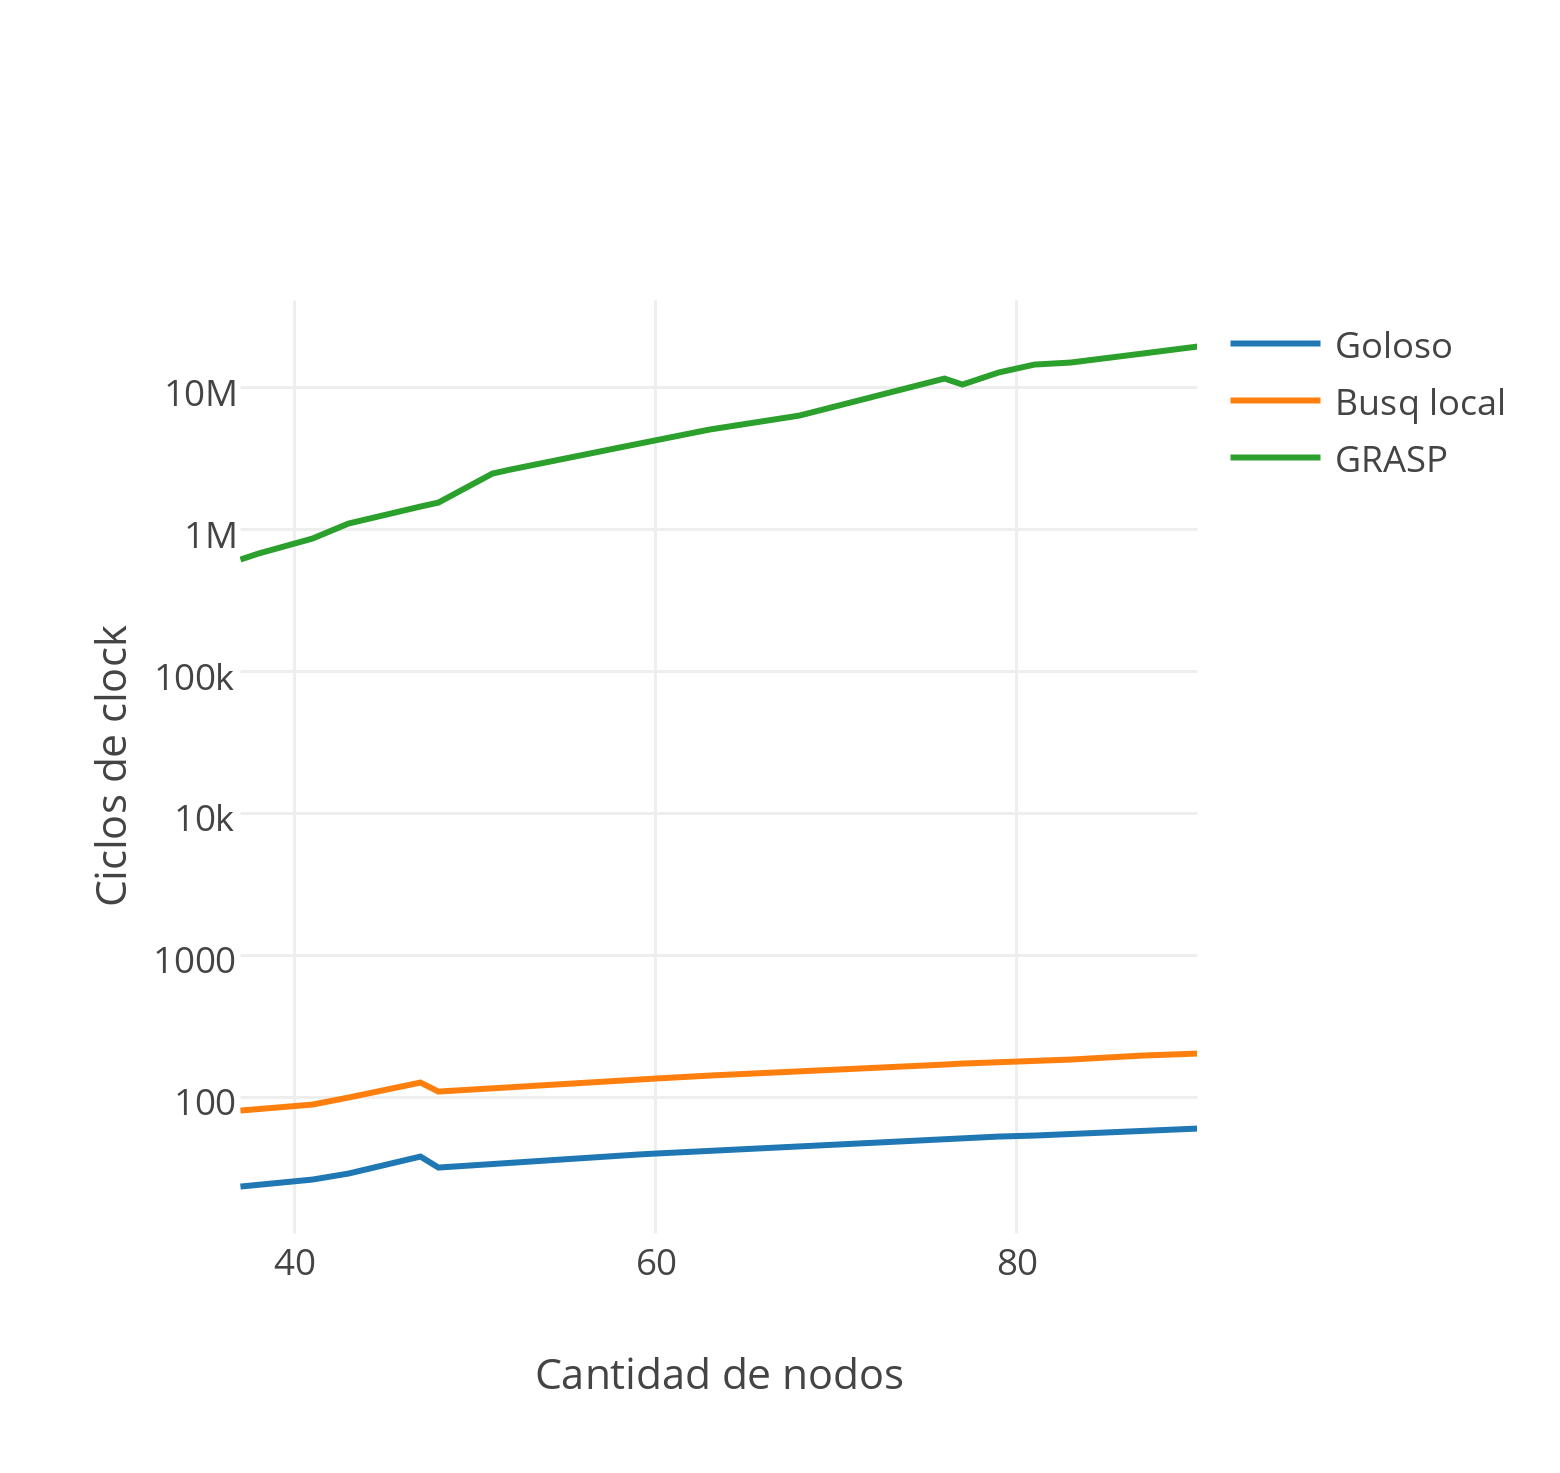
\includegraphics[scale=0.8]{imagenes/final-galaxias.png}
	\end{center}
	\caption{Comparación - Galaxias}\label{fig:5C}
\end{figure}
%\FloatBarrier

\paragraph{Calidad} 
Se ha comparado el tamaño de las soluciones obtenidas con el tamaño de la solución exacta. Los porcentajes de desaciertos sobre el total de instancias evaluadas son los siguientes:

\begin{verbatim}
Goloso: 0%
Búsqueda Local: 0%
GRASP: 0%
\end{verbatim}

Es decir, los tres algoritmos encuentran la solución exacta.

\subsubsection{Aleatorios}

Para estos experimentos se han generado dos sets de instancias $aleatorias$. Uno contiene 120 grafos de entre 4 y 15 nodos, para poder contrastar con el algoritmo exacto. El otro contiene 250 grafos de entre 16 y 40 nodos, que si bien no serán comparadas con el algoritmo exacto, posibilitará apreciar los tiempos de ejecución más ampliamente y tener una idea más general respecto a la calidad de las soluciones obtenidas.

\paragraph{Performance} Las Figuras \ref{fig:5D} y \ref{fig:5E} muestran los resultados obtenidos respecto al tiempo de ejecución para los sets 1 y 2 respectivamente. 

\subparagraph{Set 1} La Figura \ref{fig:5D} muestra que el tiempo de ejecución del algoritmo goloso es menor a los otros tres algoritmos, el tiempo de ejecución de la búsqueda local es algo mayor al goloso, y que el tiempo de ejecución de GRASP es mayor incluso al del exacto.

\subparagraph{Set 2} La Figura \ref{fig:5E} muestra claramente que el tiempo de ejecución del algoritmo goloso es menor a los otros dos algoritmos, el tiempo de ejecución de la búsqueda local es algo mayor al goloso, y que el tiempo de ejecución de GRASP es mucho mayor a los otros dos.

\begin{figure}[!htb]
\minipage{0.5\textwidth}
\begin{center}
  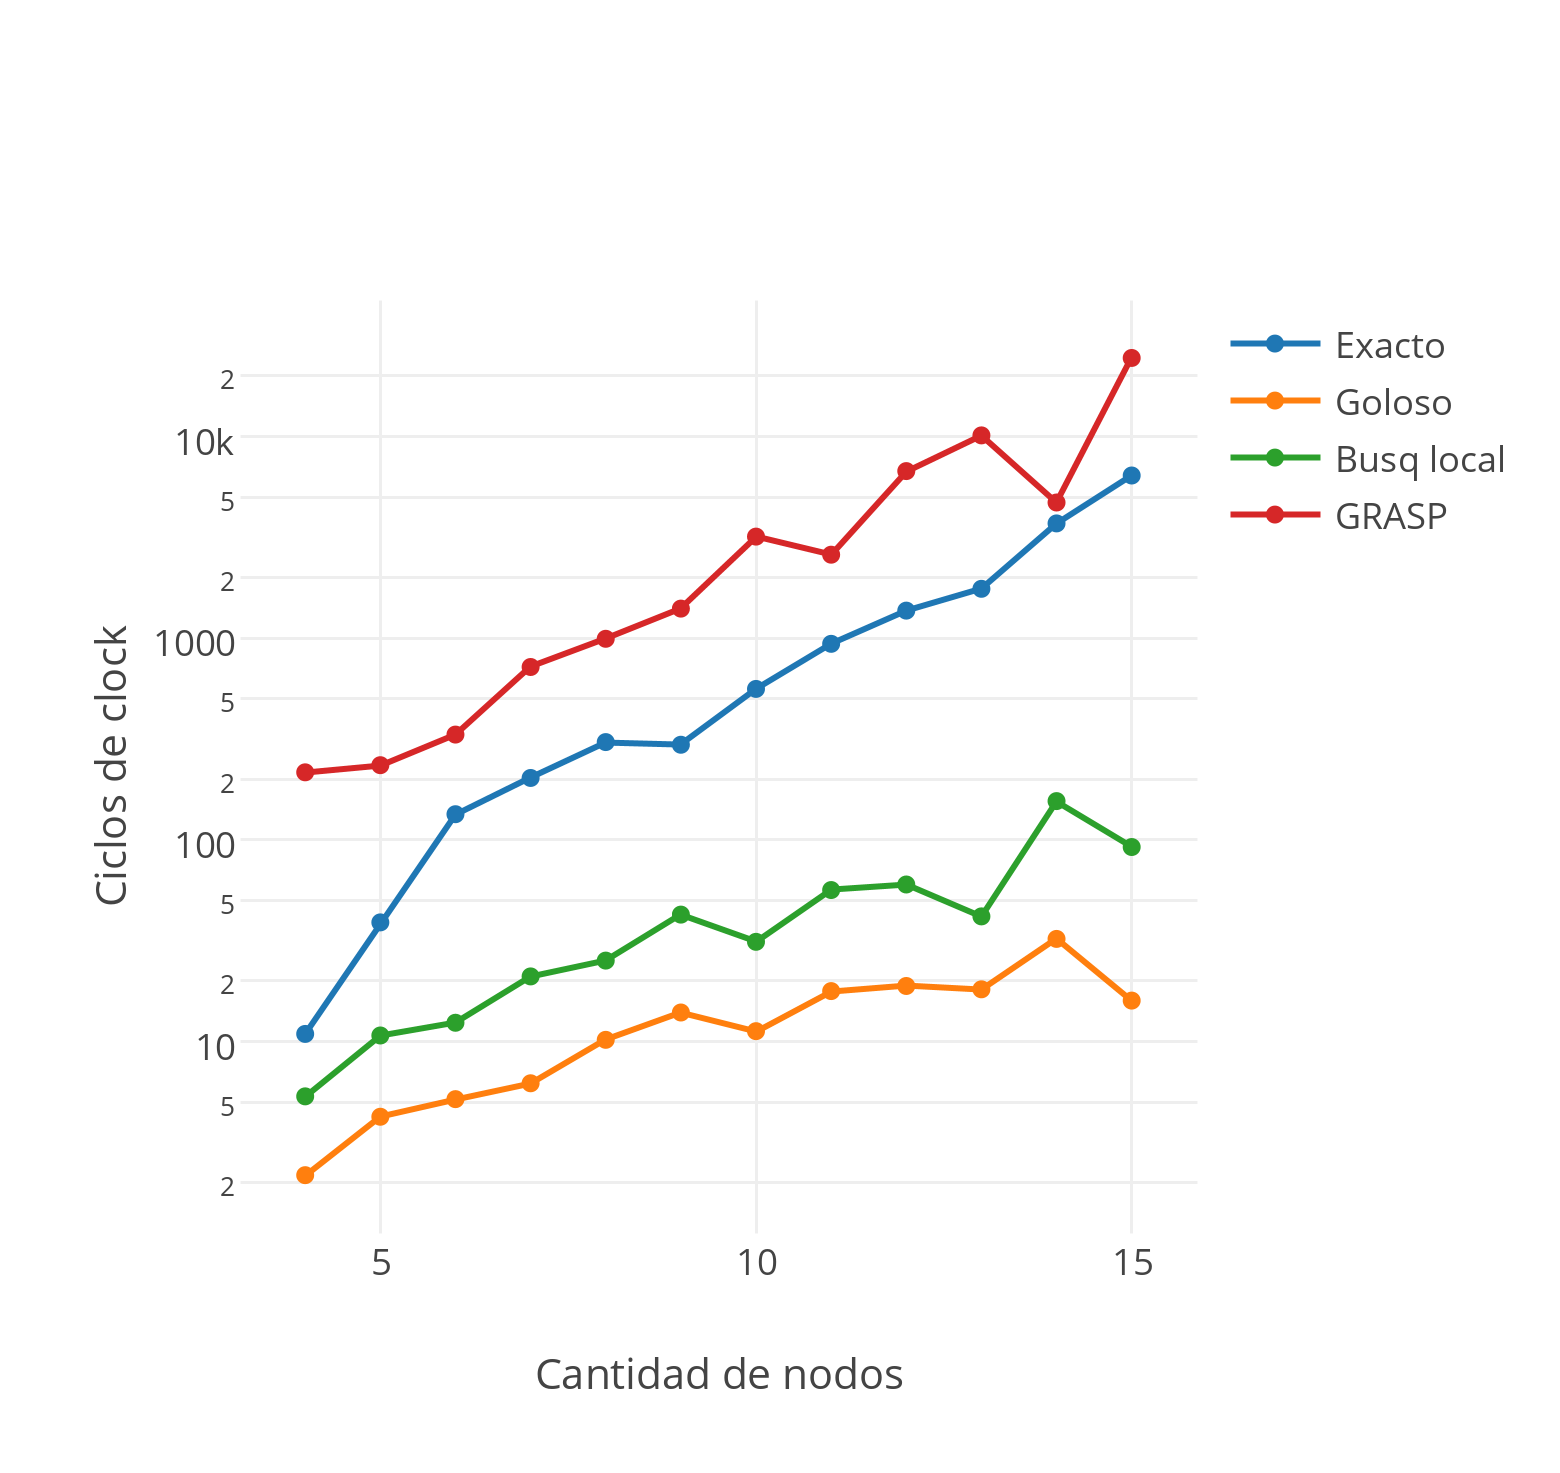
\includegraphics[scale=0.6]{imagenes/final-aleatorios-comp.png}
\end{center}
  \caption{Comparación - Aleatorios - Set 1}\label{fig:5D}
\endminipage\hfill
\minipage{0.5\textwidth}
\begin{center}
  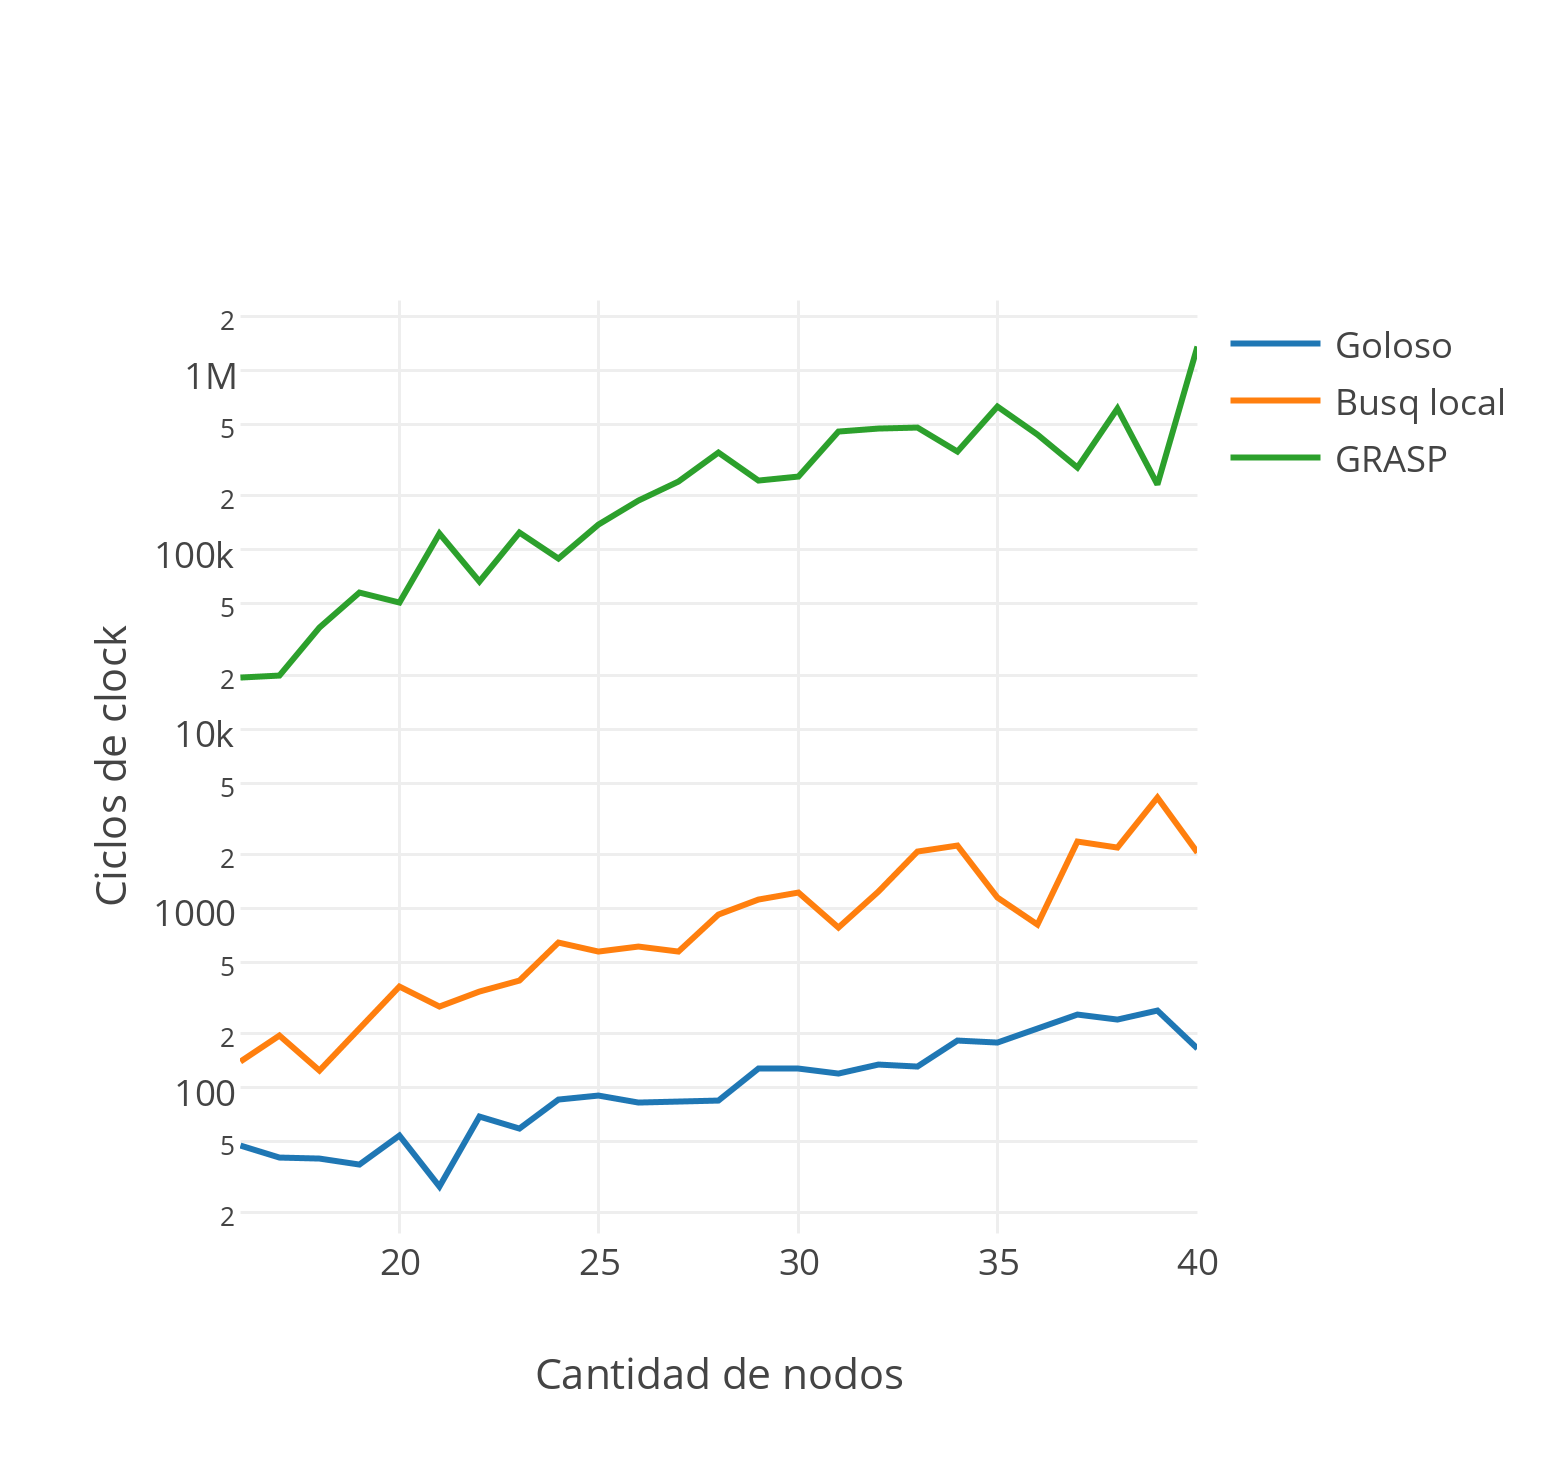
\includegraphics[scale=0.6]{imagenes/final-aleatorios.png}
\end{center}
  \caption{Comparación - Aleatorios - Set 2}\label{fig:5E}
\endminipage
\end{figure}


\paragraph{Calidad} 

\subparagraph{Set 1} Se ha comparado el tamaño de la solución obtenida con el tamaño de la solución exacta.  Los porcentajes de desaciertos sobre el total de instancias evaluadas son los siguientes:

\begin{verbatim}
Goloso: 11.67%
Búsqueda Local: 6.67%
GRASP: 0%
\end{verbatim}

Podemos observar que GRASP nuevamente tiene una tasa de error nula, búsqueda local tiene una tasa de error pequeña y el algoritmo goloso tiene una tasa de error algo mayor.

\subparagraph{Set 2} Como por el tamaño de estas instancias se dificulta la comparación con el algoritmo exacto, se consideró como la solución ``óptima'' en cada caso el menor valor obtenido entre las cuatro configuraciones, y se registró, para cada una, la cantidad de instancias en las que no se logró dicho valor. Los porcentajes de estos ``desaciertos'' sobre el total de instancias evaluadas son los siguientes:

\begin{verbatim}
Goloso: 36.8%
Búsqueda Local: 25.2%
GRASP: 1.6%
\end{verbatim}

Podemos notar que GRASP ahora tiene un mínimo porcentaje de error, búsqueda local tiene una tasa de error bastante mayor a lo visto en el Set 1, y el algoritmo goloso tiene una tasa de error algo mayor.

\subsubsection{Discusión} 

Podemos observar que en terminos de cálidad, GRASP obtiene en su amplia mayoría el mejor resultado. Sin embargo, a costa de una solución muy precisa, tiene un tiempo de ejecución más de 50 veces mayor que las otras heurísticas propuestas.
Por otro lado, Goloso en términos de performance aparece como el mejor, pero a costa de una solución poco precisa en la mayoría de los casos evaluados.
Búsqueda local se muestra con una calidad mejor a la del goloso y sin demasiado incremento en el tiempo de ejecución, pero aún así no puede compararse con GRASP en términos de calidad.
Se puede concluir entonces que de elegir alguno de estos métodos se dependerá mucho de las características de las instancias a resolver.